\documentclass{../../../../style/mkimain}

\series{2}
\month{březen}
\year{2023}

\begin{document}
\section*{II.A Polární záře}
\noindent \textbf{Úloha:}
\\
\\
V sériálu jste se dozvěděli o polární záři na Zemi, nyní se zkuste zamyslet, jak je to s polární září na naší 
sousední planetě Venuši. Rozhodněte jestli lze v atmosféře Venuše pozorovat jev podobný polární záři na Zemi, pokud ano popište, jak vzniká.
\klein
Venuše nemá vlastní magnetické pole, takže na první pohled by se mohlo zdát, že odpověď je jasná - Ne, žádný jev podobný zemské polární záři v 
atmosféře Venuše pozorovat nelze, protože nabité částice slunečního větru nemají s čím interagovat.

Tato úvaha je zcela správná, ale i přes to astronomové pozorují \emph{auroru} na Venuši.
\begin{figure}[htpb]
    \begin{center}
    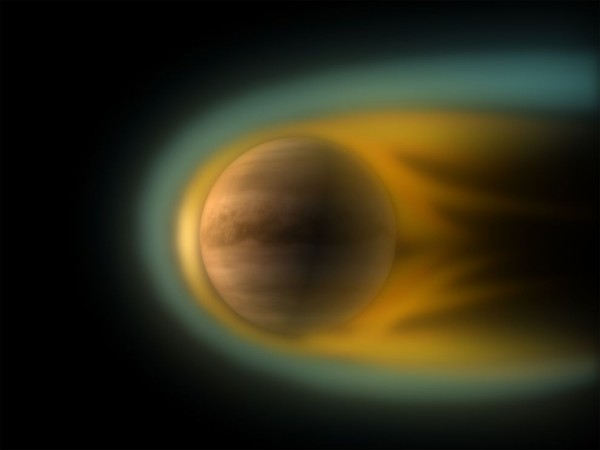
\includegraphics[width=7cm]{images/venus-aurora.jpg}
    \\
    \emph{Aurora} na Venuši\footnotemark
    \end{center}
\end{figure}
\footnotetext{Illustration by C. Carreau/ESA}
\\ Jak je to možné? V atmoféře Venuše se vyskytuje hodně iontů, převážně ionty kyslíku \ce{O^{2-}}. Plazmoid blížíce se k Venuši indukuje v 
ionosféře Venuše slabé magnetické pole. Nabité částice slunečního větru pak s tímto indukovaným polem interagují a předávájí svojí energii 
kyslíkovým iontům, které jí následně vyzáří a vytvoří tak v celé atmosféře jev podobný polární záři na Zemi. 
\end{document}
